\begin{quote}\small\textbf{观课提示}\quad 先盯住两根基向量，再预测任意格点的去向；解释矩阵为什么按列记录这些信息。

\href{https://www.youtube.com/watch?v=kYB8IZa5AuE}{原课程视频}\quad\href{https://vitael04213.github.io/3blue1brown-notes/lessons/linear-transformations.html}{本节网页与媒体}\quad\href{https://vitael04213.github.io/3blue1brown-notes/lab.html\#linear}{参数实验}
\end{quote}
\begin{figure}[htbp]\centering
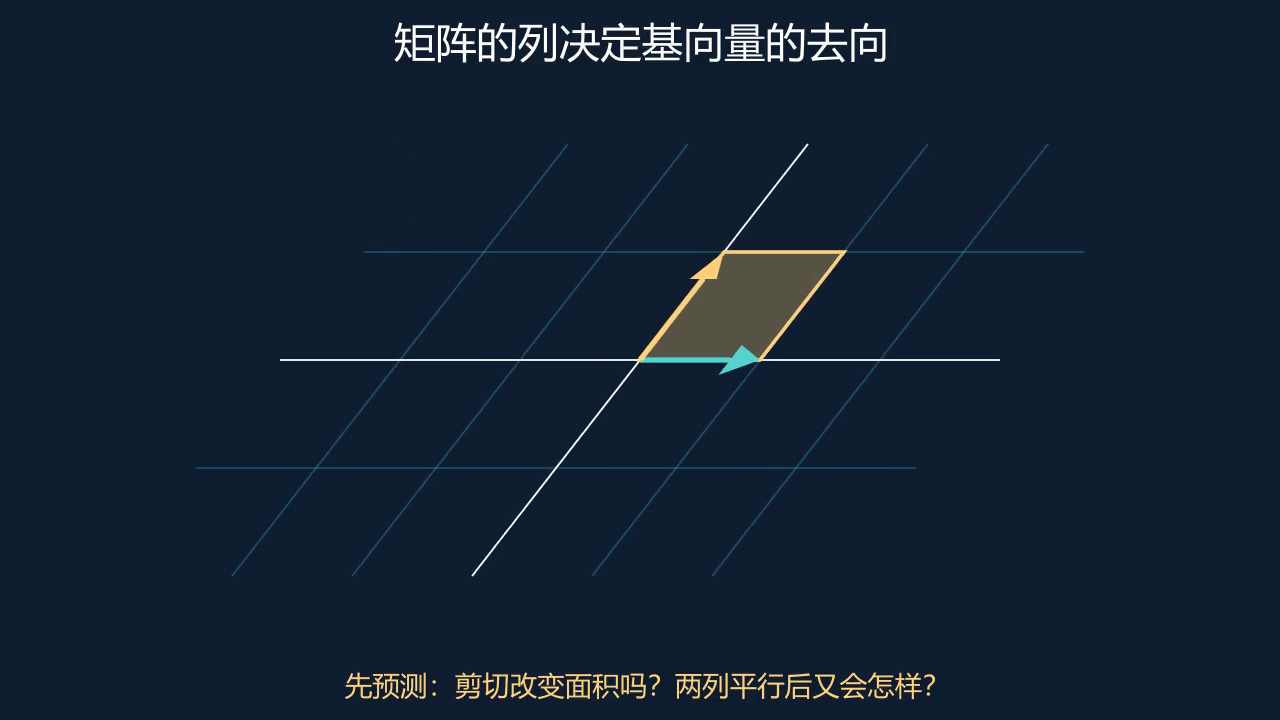
\includegraphics[width=0.98\linewidth]{figures/LinearMap.png}
\caption{剪切后的网格与单位方形。两列控制基向量去向；继续压扁时面积归零。本项目原创 Manim 动画关键帧；完整动画与操作入口见本节网页。}
\end{figure}
